\documentclass[13pt]{beamer}
\usepackage{graphicx}
\usepackage[utf8]{inputenc}
\usepackage[skip=2pt,font=scriptsize]{caption}

% Captions
\captionsetup{labelformat=empty,labelsep=none}

% References
\usepackage{url}
\bibliographystyle{acm}
\setbeamertemplate{bibliography item}[triangle]
% \usepackage{natbib}
% \setbeamertemplate{bibliography item}[text]

% Formatting
\usetheme{Singapore}
\usecolortheme{whale}

% Title Page
\title{Geometric Manifolds and the Shape of Space}
\author{Devin Delfino}
\institute{MATH 331: Geometry}
\date{Fall 2014}

% Table of Contents
\setbeamertemplate{section in toc}[sections numbered]
\setbeamercolor{alerted text}{fg=blue}
\AtBeginSection[]
{
  \begin{frame}
    \frametitle{Outline}
    \tableofcontents[currentsection]
  \end{frame}
}

\begin{document}
% TITLE ------------------------------------------------
\frame{\titlepage}

% Table of Contents ------------------------------------------------
\begin{frame}
\frametitle{Outline}
\tableofcontents
\end{frame}

\section{Geometric 2-Manifolds} % ==========================================================================
% 2-MANIFOLDS ------------------------------------------------
\begin{frame}
\frametitle{Introduction}
	\begin{itemize}
		\item A \alert{Geometric 2-Manifold} is a connected surface that is locally isometric to either the Euclidean plane, hyperbolic plane, or sphere.
		\item Cones (excluding cone point), Cylinders, and Tori are examples of flat 2-manifolds
    % \item The double torus is a 2-manifold that is locally isometric to the hyperbolic plane
	\end{itemize}
	\begin{columns}[r] % the "c" option specifies center vertical alignment
    \column{1\textwidth} % column designated by a command
     \centering
      \begin{figure}
        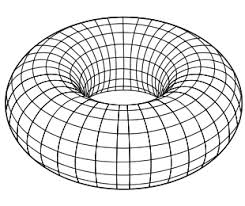
\includegraphics[height=2cm]{./img/torus}
        \caption{http://commons.wikimedia.org/wiki/File:Simple\_Torus.svg}
      \end{figure}
    % \column{.3\textwidth}
    %  \centering
    %  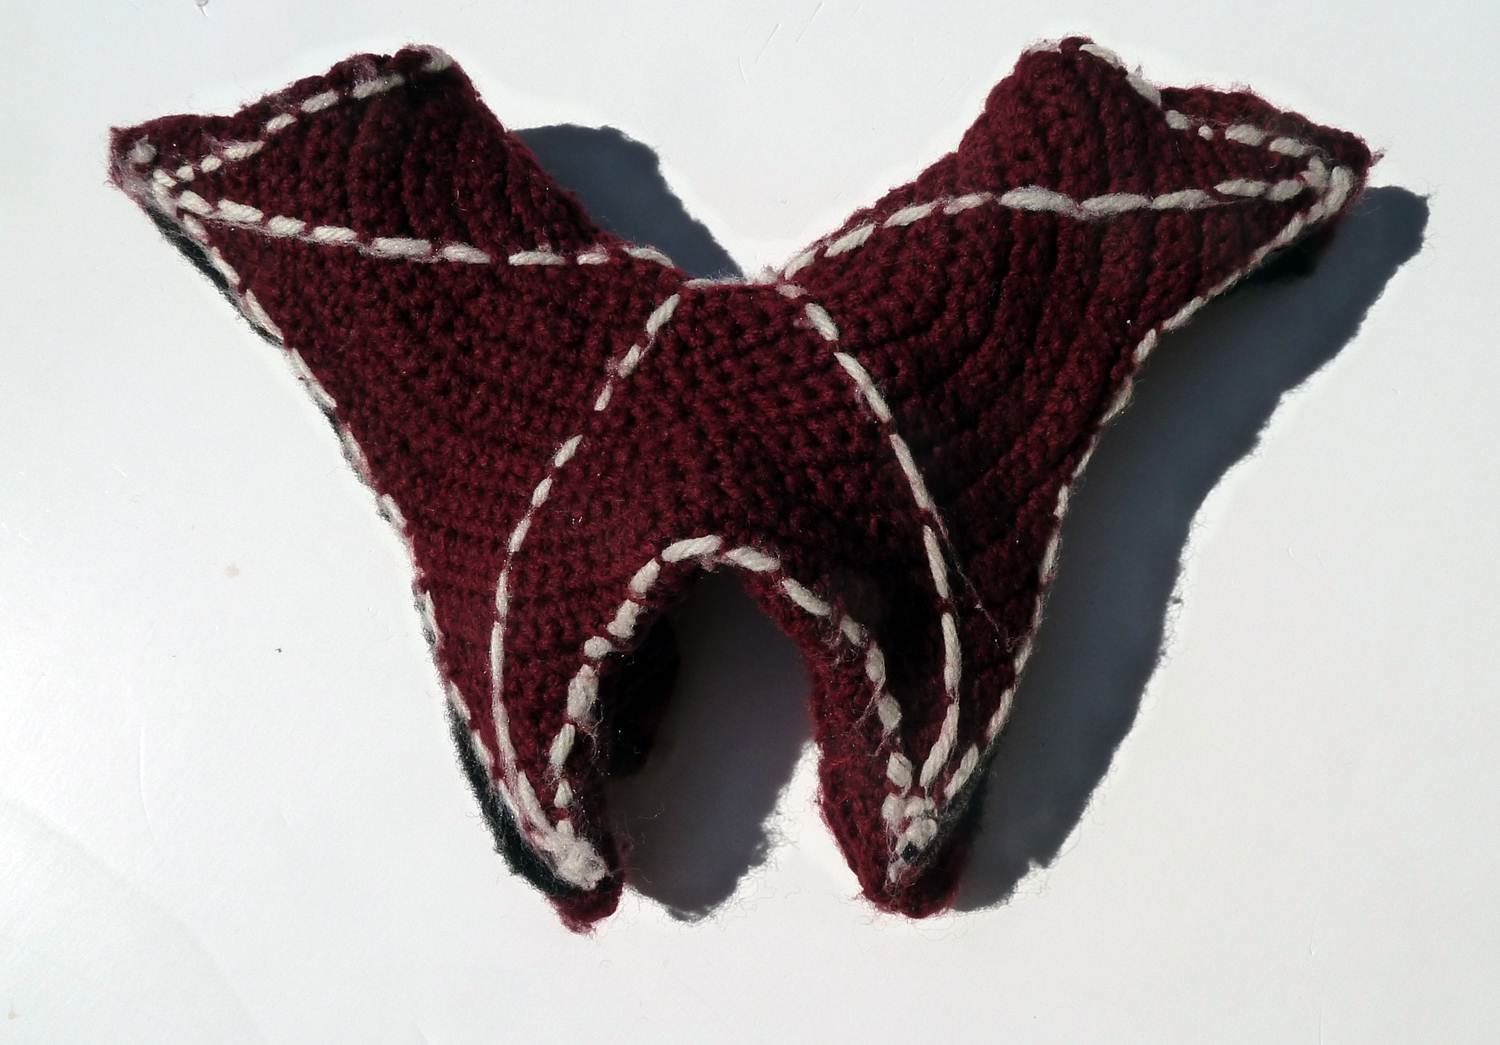
\includegraphics[height=2cm]{./img/hyperbolicpants}
    % \column{.3\textwidth}
    %  \centering
    %  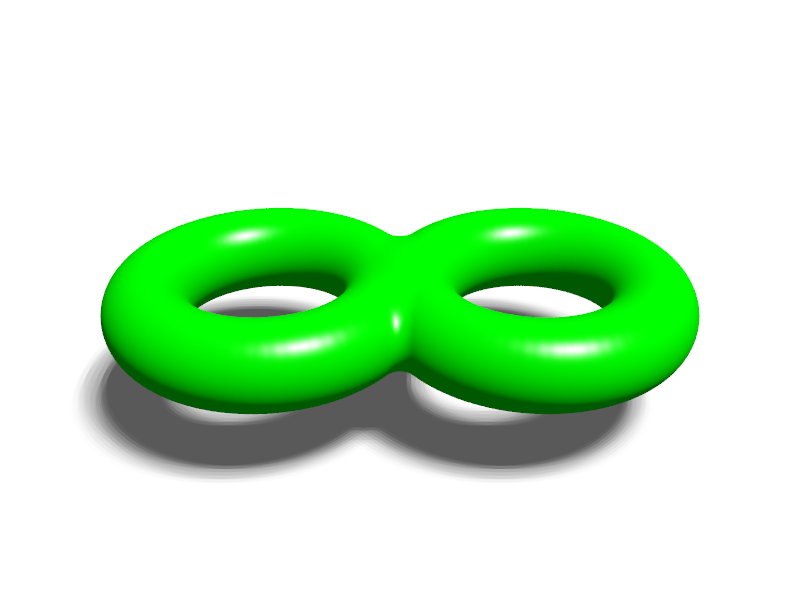
\includegraphics[height=2cm]{./img/doubletorus}
  \end{columns}
	%torus, hyperbolic pants, double torus
\end{frame}

% GLUINGS ------------------------------------------------
\begin{frame}
\frametitle{Gluings}
	\begin{itemize}
    \item \alert{Gluings} are when two edges or sides of a surface are ``connected'' and share the same set of points.
		\item The orientation of the gluings determine the structure of the manifold and whether it is flat, hyperbolic, or spherical.
	\end{itemize}

  \begin{columns}[r] % the "c" option specifies center vertical alignment
    \column{.5\textwidth} % column designated by a command
     \centering
      \begin{figure}
        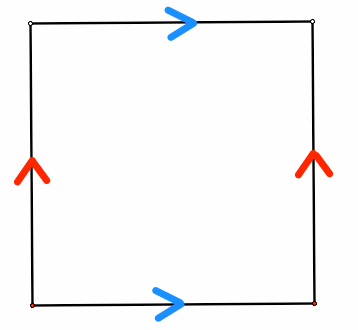
\includegraphics[height=3cm]{./img/torusgluing}
      \end{figure}
    \column{.5\textwidth}
     \centering
      \begin{figure}
        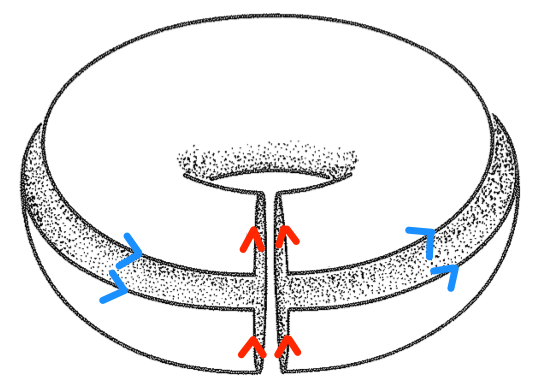
\includegraphics[height=3cm]{./img/torusconstruction}
        \caption{The Shape of Space - Figure 7.14, pg. 117}
      \end{figure}
     % page 117 lower figure of shape of space
    % \column{.3\textwidth}
    %  \centering
    %   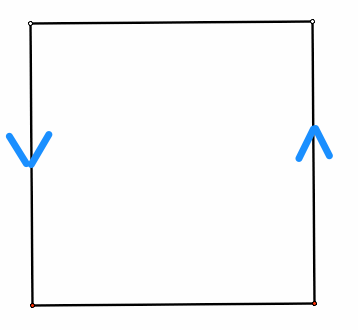
\includegraphics[height=3cm]{./img/mobiusgluing}
  \end{columns}
\end{frame}

\section{Geometric 3-Manifolds} % ==========================================================================
% 3-MANIFOLDS ------------------------------------------------
\begin{frame}
\frametitle{Geometric 3-Manifolds}
  \begin{itemize}
    \item A \alert{Geometric 3-Manifold} is a space where the region surrounding any point is isometric to Euclidean 3-space, hyperbolic 3-space, or the 3-sphere.
    \item \alert{Euclidean 3-space} is formed by adding a third dimension to the plane.
    \item \alert{Hyperbolic 3-space} is formed by adding a third dimension to the hyperbolic plane.
    \item \alert{The 3-Sphere} is the set of points in 4-D space that are an equal distance away from an origin.
  \end{itemize}
  \begin{columns}[r] % the "c" option specifies center vertical alignment
    \column{.5\textwidth} % column designated by a command
     \centering
      \begin{figure}
        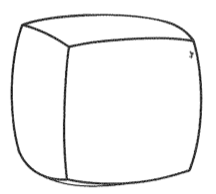
\includegraphics[height=2.70cm]{./img/cube3sphere}
        \caption{The Shape of Space - Figure 14.7, pg. 209}
      \end{figure}
    \column{.5\textwidth}
     \centering
      \begin{figure}
        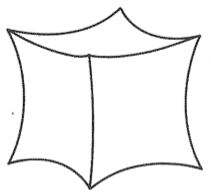
\includegraphics[height=2.70cm]{./img/cubeH3}
        \caption{The Shape of Space - Figure 15.2, pg. 215}
      \end{figure}
     % page 209, 215
  \end{columns}
\end{frame}

% 3-TORUS ------------------------------------------------
\begin{frame}
\frametitle{3-Torus}
  \begin{itemize}
    \item The \alert{3-Torus} is:
          \begin{itemize}
             \item Constructed by gluing opposite sides of a cube.
             \item A geometric 3-manifold that is isometric to Euclidean 3-space.
           \end{itemize} 
    \item Cubes perfectly fill 3-space (8 cubes meet at each corner).
  \end{itemize}
  \begin{columns}[r] % the "c" option specifies center vertical alignment
    \column{1\textwidth} % column designated by a command
     \centering
      \begin{figure}
        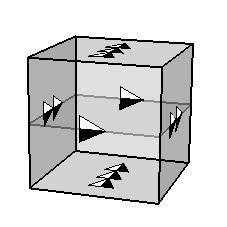
\includegraphics[height=4cm]{./img/cubegluing}
        \caption{http://euler.slu.edu/escher/index.php/The\_Three\_Geometries}
      \end{figure}
    % \column{.5\textwidth}
    %  \centering
    %  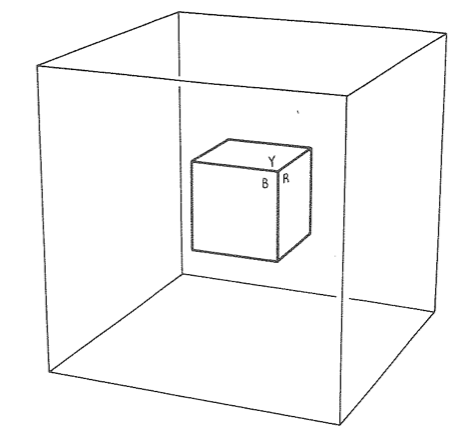
\includegraphics[height=4cm]{./img/torus3} % page 106
  \end{columns}
\end{frame}


% show curved space application

% INSIDE THE 3-TORUS ------------------------------------------------
% \begin{frame}
% \frametitle{Inside the 3-Torus}
%   \begin{columns}[c] % the "c" option specifies center vertical alignment
%     \column{1\textwidth}
%      \centering
%      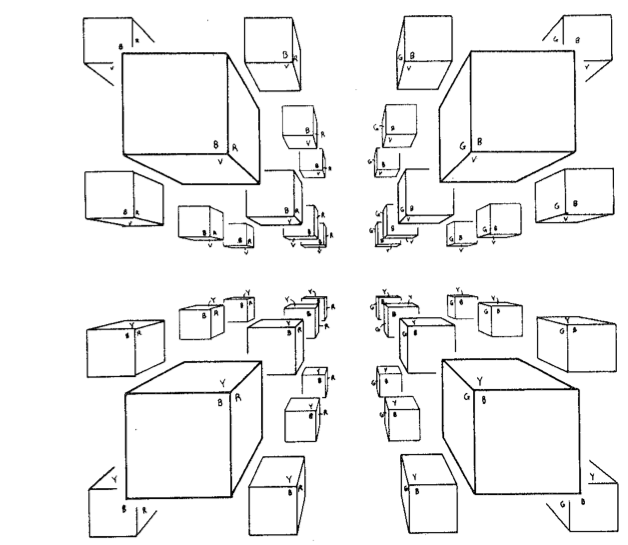
\includegraphics[height=7cm]{./img/inside3torus}
%   \end{columns}
% \end{frame}

% POINCARE SPACE ------------------------------------------------
\begin{frame}
\frametitle{Poincar\'e Dodecahedral Space}
  \begin{itemize}
    \item \alert{Poincar\'e Dodecahedral Space} is:
          \begin{itemize}
             \item Constructed by gluing opposite sides of a dodecahedron with a clockwise $\frac{1}{10}$ rotation.
             \item A geometric 3-manifold that is isometric to the 3-Sphere.
           \end{itemize} 
  \end{itemize}

  \begin{columns}[c] % the "c" option specifies center vertical alignment
    \column{1\textwidth}
     \centering
      \begin{figure}
        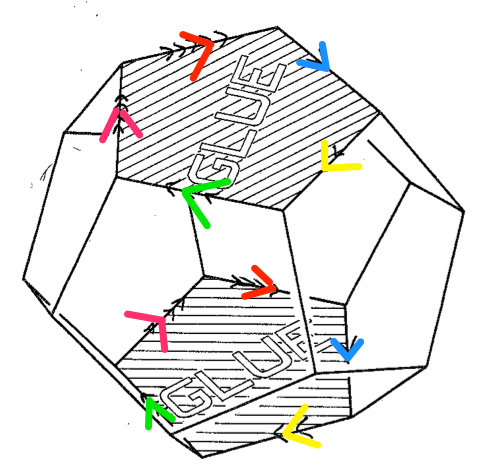
\includegraphics[height=5cm]{./img/one_tenth}
        \caption{The Shape of Space - Figure 16.3, pg. 222}
      \end{figure}
  \end{columns}
\end{frame}

% POINCARE SPACE ------------------------------------------------
\begin{frame}
\frametitle{Poincar\'e Dodecahedral Space, cont.}
  \begin{itemize}
    \item Four dodecahedrons meet at each vertex, and the angles are too small to perfectly fill 3-Space.
    \item In the 3-Sphere, as the dodecahedrons expand, the angles increase and eventually fit together in groups of four.
  \end{itemize}

  \begin{columns}[c] % the "c" option specifies center vertical alignment
    \column{1\textwidth}
     \centering
      \begin{figure}
        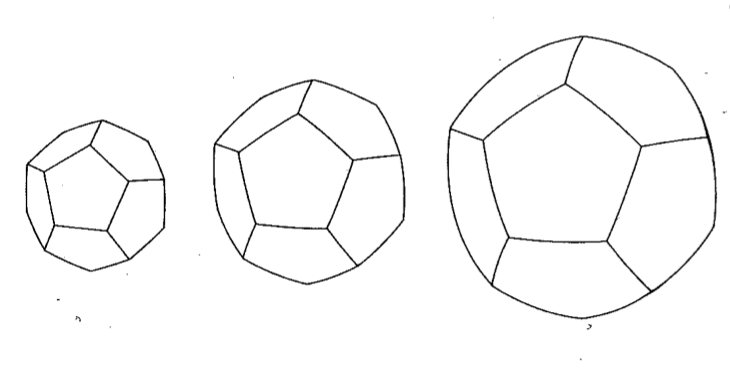
\includegraphics[height=5cm]{./img/poincarespace}
        \caption{The Shape of Space - Figure 16.4, pg. 223}
      \end{figure}
  \end{columns}
\end{frame}

%SHOW MODEL

% SEIFERT-WEBER SPACE ------------------------------------------------
\begin{frame}
\frametitle{Seifert-Weber Space}
  \begin{itemize}
    \item \alert{Seifert-Weber Space} is:
          \begin{itemize}
             \item Constructed by gluing opposite sides of a dodecahedron with a clockwise $\frac{3}{10}$ rotation.
             \item A geometric 3-manifold that is isometric to Hyperbolic 3-Space.
           \end{itemize} 
  \end{itemize}

  \begin{columns}[c] % the "c" option specifies center vertical alignment
    \column{1\textwidth}
     \centering
      \begin{figure}
        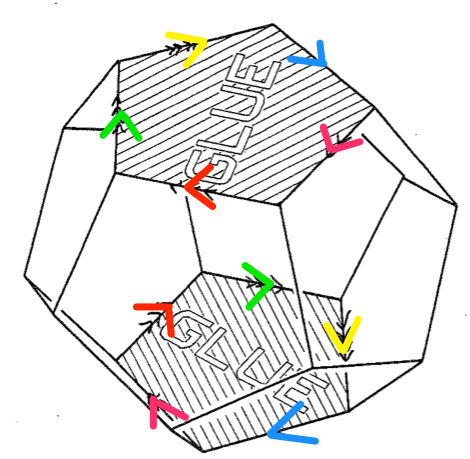
\includegraphics[height=4.75cm]{./img/three_tenths}
        \caption{The Shape of Space - Figure 16.1, pg. 220}
      \end{figure}
  \end{columns}
\end{frame}

% SEIFERT-WEBER SPACE ------------------------------------------------
\begin{frame}
\frametitle{Seifert-Weber Space, cont.}
  \begin{itemize}
    \item 20 dodecahedrons meet at each vertex, and the angles are too large to perfectly fill 3-Space.
    \item In Hyperbolic 3-Space, as the dodecahedrons expand, the angles decrease and eventually fit together in groups of twenty.
  \end{itemize}

  \begin{columns}[c] % the "c" option specifies center vertical alignment
    \column{1\textwidth}
     \centering
      \begin{figure}
        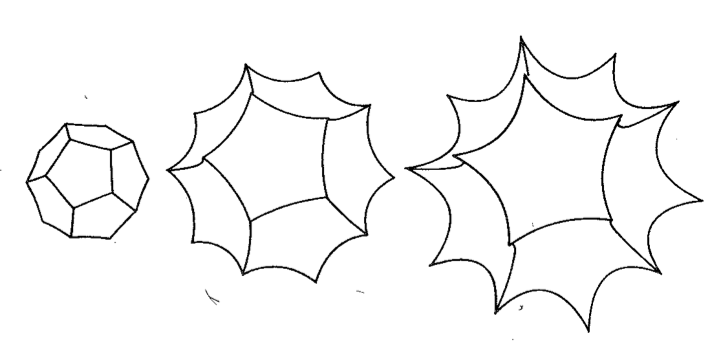
\includegraphics[height=5cm]{./img/seifertspace}
        \caption{The Shape of Space - Figure 16.2, pg. 221}
      \end{figure}
  \end{columns}
\end{frame}

% SHOW SPACE

\section{The Shape of Space} % ==========================================================================
% CMB ------------------------------------------------
\begin{frame}
\frametitle{Cosmic Microwave Background}
  \begin{itemize}
    \item Following the Big Bang, radiation scattered throughout the Universe.
    \item As the Universe expanded overtime, this radiation has cooled to microwaves known as \alert{Cosmic Microwave Background (CMB)}.

    \begin{columns}[c] % the "c" option specifies center vertical alignment
    \column{1\textwidth}
     \centering
      \begin{figure}
        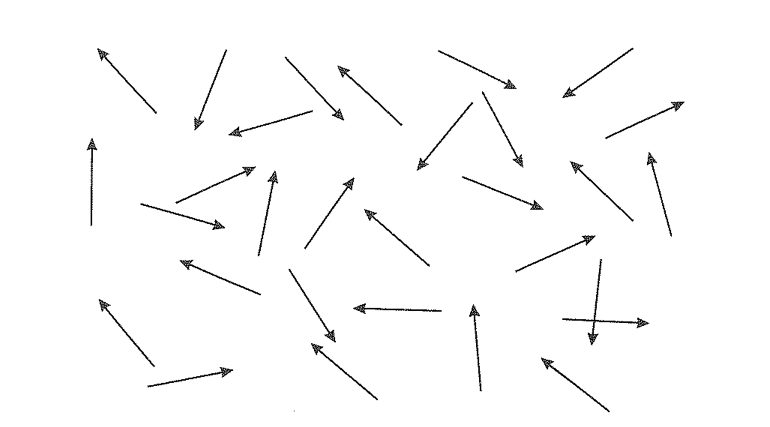
\includegraphics[height=4.75cm]{./img/cmbwaves} %page 300
        \caption{The Shape of Space - Figure 22.5, pg. 300}
      \end{figure}
  \end{columns}

  \end{itemize}
\end{frame}

% CMB ------------------------------------------------
\begin{frame}
\frametitle{Cosmic Microwave Background, cont.}
  \begin{itemize}
    \item Microwaves are nearly uniform in temperature
    \item Small fluctuations in temperature due to the density of the region where they formed.
    \item Microwaves travel in all directions.
    \item First observed in 1965 by Arno Penzias and Robert Wilson of Bell Labs.
  \end{itemize}
  % Interesting properties of CMB include:
    %       \begin{itemize}
    %         \item Nearly uniform temperature with only small fluctuations.
    %         \item Distributed evenly throughout space.
    %         \item Travels in all directions
    %       \end{itemize}

    \begin{columns}[c] % the "c" option specifies center vertical alignment
    \column{1\textwidth}
     \centering
      \begin{figure}
        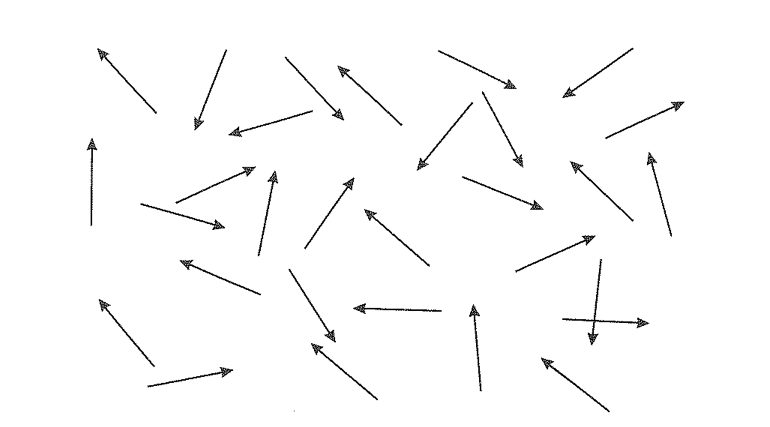
\includegraphics[height=4cm]{./img/cmbwaves} %page 300
        \caption{The Shape of Space - Figure 22.5, pg. 300}
      \end{figure}
  \end{columns}

\end{frame}

% LSS ------------------------------------------------
\begin{frame}
\frametitle{Last Scattering Surface}
  \begin{itemize}
    \item Microwaves that we observe from Earth have travelled the same distance from their starting position to the time we record them.
    \item All microwaves observed at one time originated on the surface of the \alert{Last Scattering Sphere (LSS)}.
    % \item The LSS is unique to the observer, so viewing from Earth, Earth is at the center of its LSS.
    % \item There are slight fluctuations in the temperature of the CMB due to the differences in densities of their starting positions.
  \end{itemize}

  \begin{columns}[c] % the "c" option specifies center vertical alignment
    \column{1\textwidth}
     \centering
      \begin{figure}
        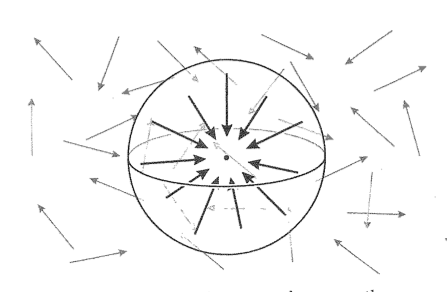
\includegraphics[height=4.5cm]{./img/scattering} %page 301
        \caption{The Shape of Space - Figure 22.6, pg. 301}
      \end{figure}
  \end{columns}
\end{frame}

% LSS ------------------------------------------------
\begin{frame}
\frametitle{The Shape of Space}
  \begin{itemize}
    \item Assuming the Universe is a 3-Manifold, there exists reoccuring images of the Earth at the center of its LSS.
    \item If the LSS is larger than a single image of the Universe, then it overlaps itself.
  \end{itemize}

  \begin{columns}[c] % the "c" option specifies center vertical alignment
    \column{1\textwidth}
     \centering
      \begin{figure}
        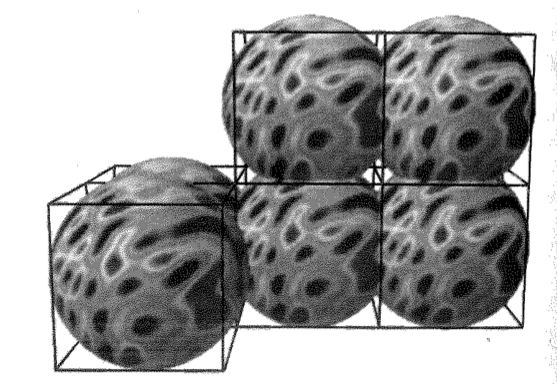
\includegraphics[height=4.5cm]{./img/LssIntersecting} %page 359 - Experiencing Geo 
        \caption{The Shape of Space - Figure 22.8, pg. 304}
      \end{figure}
  \end{columns}
\end{frame}

% SHAPE OF SPACE ------------------------------------------------
\begin{frame}
\frametitle{The Shape of Space, cont.}
  \begin{itemize}
    \item In the case of the 3-Torus Universe, circles form along each side of the cube where the LSS overlaps itself.
    \item The circles on opposite sides contain the same set of CMB, which produce the same temperature pattern.
  \end{itemize}

  \begin{columns}[c] % the "c" option specifies center vertical alignment
    \column{1\textwidth}
     \centering
      \begin{figure}
        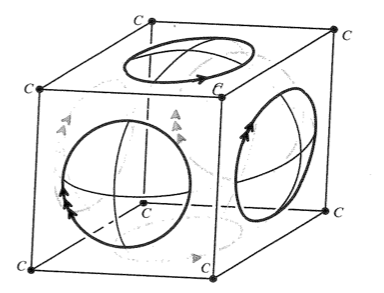
\includegraphics[height=4.5cm]{./img/shapeofspace} 
        \caption{Experiencing Geometry- Figure 24.8, pg. 359}
      \end{figure}
  \end{columns}
\end{frame}

% CONCLUSION ------------------------------------------------
\begin{frame}
\frametitle{Conclusion}
  \begin{itemize}
    \item The orientation of the temperature patterns of these sets hint at the gluings of the 3-Manifold Universe, and ultimately the geometric structure.
    \item NASA's Wilkinson Microwave Anisotropy Probe (WMAP) mapped out the CMB and its temperature patterns.
    \item Results showed that Universe should hold properties similar to Euclidean Geometry
  \end{itemize}

  \begin{columns}[c] % the "c" option specifies center vertical alignment
      \column{1\textwidth}
       \centering
        \begin{figure}
          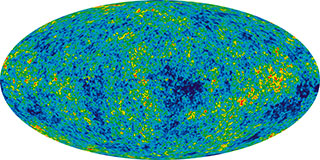
\includegraphics[height=3.5cm]{./img/cmbsky} 
          \caption{http://map.gsfc.nasa.gov/media/121238/index.html}
        \end{figure}
    \end{columns}
\end{frame}

% QUESTIONS ------------------------------------------------
\begin{frame}
\frametitle{Questions?}
   \begin{columns}[c] % the "c" option specifies center vertical alignment
    \column{.5\textwidth}
     \centering
      \begin{figure}
        \includegraphics[height=4cm]{./img/3torusEarth} % shape of space cover
        \caption{http://web.math.princeton.edu/\\conference/Thurston60th/lectures.html}
      \end{figure}
    \column{.5\textwidth}
     \centering
      \begin{figure}
        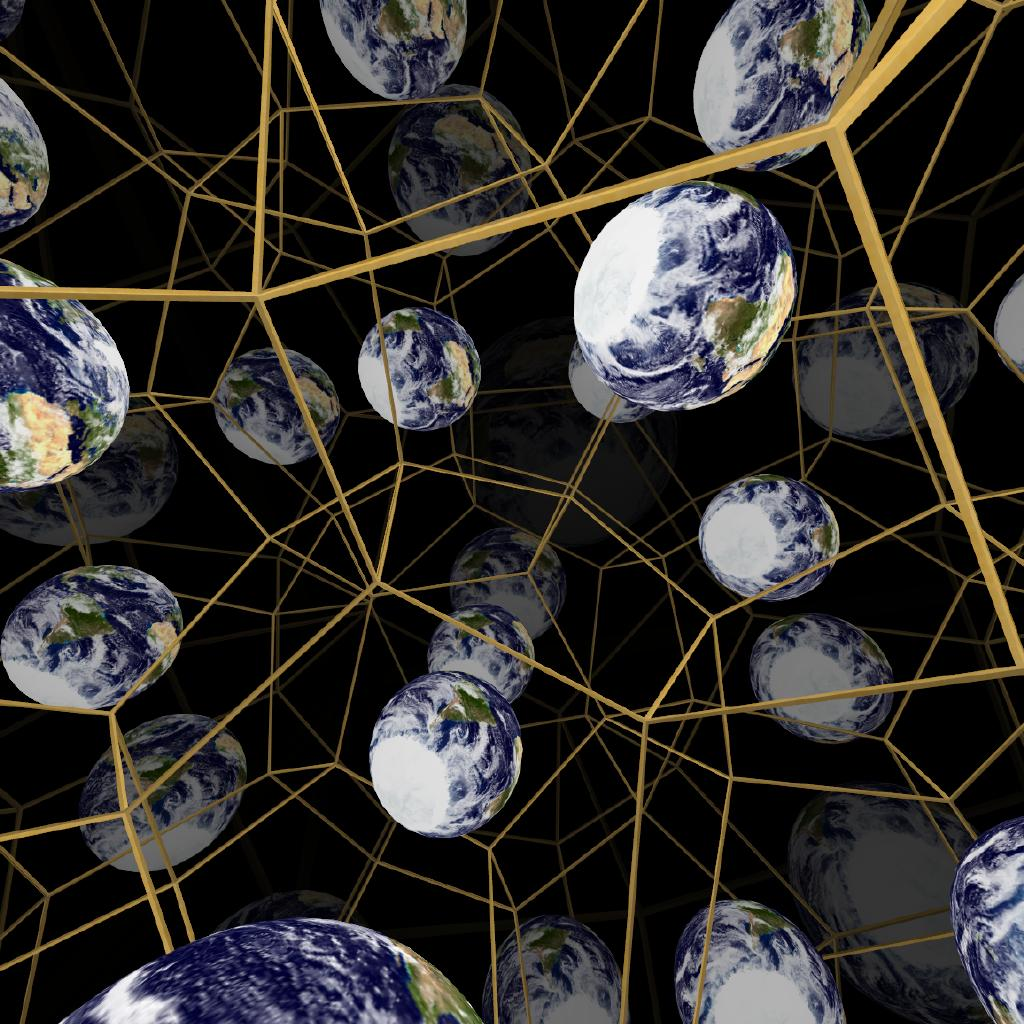
\includegraphics[height=4cm]{./img/poincarespaceEarth} % wraparound universe cover
        \caption{http://quibb.blogspot.com/2011/05/\\manifolds-shape-of-universe-iii.html}
      \end{figure}
  \end{columns}
\end{frame}

% References ------------------------------------------------
 \begin{frame}[allowframebreaks]
  \frametitle{References}
  \nocite{*} 
  \bibliography{workscited}
  % \bibliography{ShapeOfSpace,WraparoundUniverse,ExperiencingGeo,NASA}
\end{frame}

\end{document}